\documentclass[tikz,border=6pt]{standalone}
\usepackage[T1]{fontenc}
\usepackage[utf8]{inputenc}
\usepackage{pgfplots}
\usepgfplotslibrary{groupplots}
\usetikzlibrary{calc}
\pgfplotsset{compat=1.18}
\begin{document}
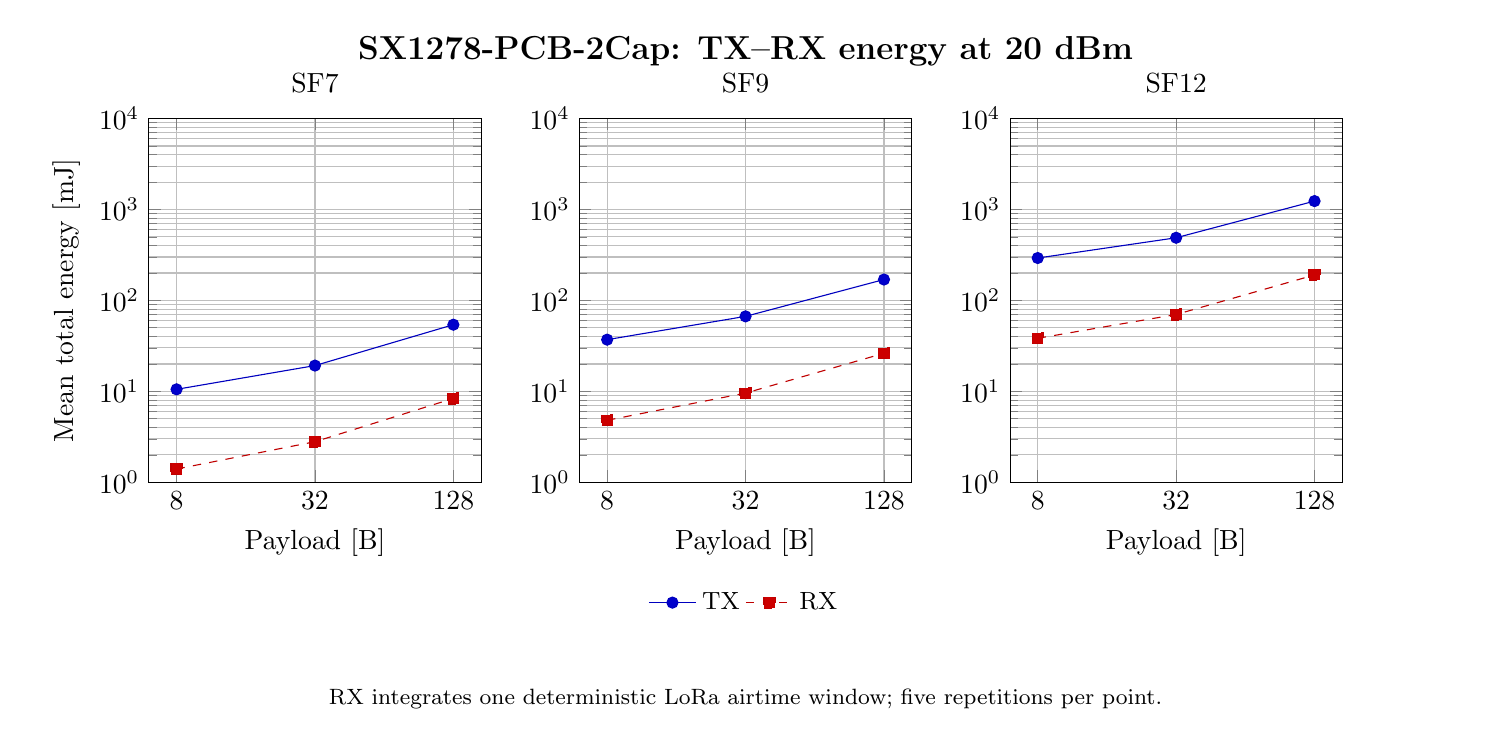
\begin{tikzpicture}
\begin{groupplot}[/pgf/number format/use comma, group style={group size=3 by 1, horizontal sep=1.25cm},
  width=5.8cm,height=6.2cm,xmode=log,log basis x=2,ymode=log,log basis y=10,ymin=1,ymax=10000,
  xtick={8,32,128},xticklabels={8,32,128},grid=both,xlabel={Payload [B]},
  legend style={draw=none,fill=none,font=\small,at={(0.5,-0.27)},anchor=north,legend columns=-1}]
% TX--RX energy
\nextgroupplot[title={SF7},ylabel={Mean total energy [mJ]}]
\addplot+[blue!75!black,solid,mark=*,error bars/.cd,y dir=both,y explicit] coordinates {(8,10.5149778) +- (0,0.0448558818) (32,19.1972084) +- (0,0.0789783074) (128,54.0580208) +- (0,0.245531543)};
\addplot+[red!75!black,dashed,mark=square*,error bars/.cd,y dir=both,y explicit] coordinates {(8,1.39764856) +- (0,0.00312146879) (32,2.78976214) +- (0,0.00455151495) (128,8.35350897) +- (0,0.0228838987)};
\nextgroupplot[title={SF9}]
\addplot+[blue!75!black,solid,mark=*,error bars/.cd,y dir=both,y explicit] coordinates {(8,37.0048645) +- (0,0.220095035) (32,66.7473383) +- (0,0.375907224) (128,169.713111) +- (0,0.688965257)};
\addlegendentry{TX}
\addplot+[red!75!black,dashed,mark=square*,error bars/.cd,y dir=both,y explicit] coordinates {(8,4.79952176) +- (0,0.0100938768) (32,9.56313079) +- (0,0.0172105171) (128,26.2076347) +- (0,0.0552717097)};
\addlegendentry{RX}
\nextgroupplot[title={SF12}]
\addplot+[blue!75!black,solid,mark=*,error bars/.cd,y dir=both,y explicit] coordinates {(8,292.537555) +- (0,0.588519522) (32,488.72549) +- (0,0.595746087) (128,1237.13689) +- (0,2.3561846)};
\addplot+[red!75!black,dashed,mark=square*,error bars/.cd,y dir=both,y explicit] coordinates {(8,38.3035689) +- (0,0.064805891) (32,70.0016209) +- (0,0.0753069932) (128,190.581705) +- (0,0.125091748)};
\end{groupplot}
\node[font=\bfseries\large] at ($(group c2r1.north)+(0,0.85cm)$) {SX1278-PCB-2Cap: TX--RX energy at 20 dBm};
\node[font=\footnotesize,align=center,text width=18cm] at ($(group c2r1.south)+(0,-2.75cm)$) {RX integrates one deterministic LoRa airtime window; five repetitions per point.};
\end{tikzpicture}
\end{document}
